\section{Wzroce projektowe (3) - czynnościowe }
\subsection{Polecenie (ang. command)}
Polecenie umożliwia zamianę żądania w samodzielny, osobny obiekt. Z tym wzorcem często można się spotkać w kontekście interfejsów użytkownika. Do dane przycisku może być przypisana akcja (obiekt implementujący interfejs \texttt{ICommand}).  Po kliknięciu w dany element, instancja przycisku nie jest świadoma akcji, która się powinna wykonać. Pozwala to łatwą zmianę działania przycisku i umożliwia zachowanie zasady pojedynczej odpowiedzialności (komponent odpowiedzialny za interfejs graficzny nie jest świadomy działania logiki biznesowej). Obiekty polecenia łączą te dwie warstwy. Dodatkowo chcąc wprowadzić nową funkcjonalność wystarczy stworzyć nowy obiekt implementujący \texttt{ICommand} i przekazać go do nadawcy (zasada otwarte/zamknięte).

Jeśli obiekt polecenia do wykonania żądania wymaga dodatkowych parametrów (np. z pól formularza), należy je przekazać jako argument konstruktora (jeśli obiekt ma być niezmienny) albo przez jego właściwości.

Co więcej wykorzystanie wzorca Polecenie pozwala na przypisanie kilku przyciskom tej samej czynności np. operacja zapisywania może być dostępna zarówno jako osobny przycisk jak i kombinacja klawiszy \texttt{Ctrl+S}.

Dodatkowo omawiany wzorzec pozwala na implementacje cofania, ponawiania operacji oraz kolejkowania. Można również wiele kilka prostych poleceń łączyć w jedno bardziej skomplikowane.

Obiekt przycisku powinien posiadać pole/właściwość typu \texttt{ICommand}, można ją przekazać np. jako argument konstruktora. 


%Innym podejściem mogłoby być stworzenie wielu klas dziedziczących po klasie Button np. OkButton, CancelButton, ApplyButton itp...

%Warto zwrócić uwagę na wzorzec MVVM i jak Microsoft podszedł do tematu obłsugi przycisków UI


%PRZYKŁAD Z REFACTORING GURU: Podczas długiego spaceru po mieście, docierasz do miłej restauracji i siadasz przy oknie. Przyjazny kelner szybko przyjmuje zamówienie, spisując je na małym kawałku papieru. Następnie kelner idzie do kuchni i przykleja kartkę na ścianie. Po jakimś czasie zamówienie dociera do szefa kuchni, który przygotowuje danie, a następnie umieszcza posiłek na tacce wraz z zamówieniem. Kelner znajduje tackę, sprawdza zgodność z zamówieniem i zanosi ją do stolika. Zamówienie na papierze stanowi polecenie. Trafia do kolejki, do momentu aż szef kuchni je przygotuje. Zamówienie zawiera wszystkie niezbędne informacje wymagane do przygotowania posiłku. Umożliwia to kucharzowi rozpoczęcie gotowania od razu, zamiast ustalać szczegóły z klientem na własną rękę.


\begin{figure}[hbt!]
	\centering
	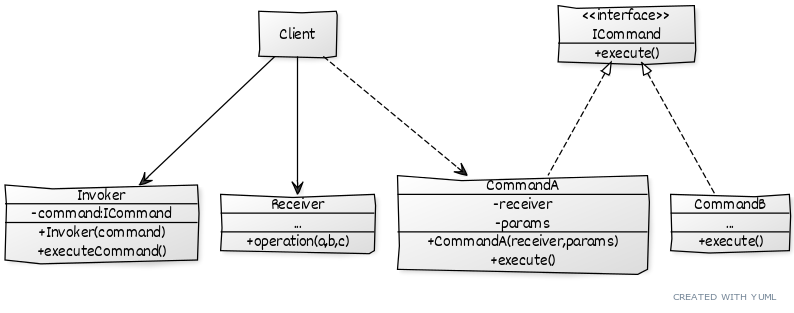
\includegraphics[width=0.9\linewidth]{images/CommandUml}
	\caption{Diagram UML wzorca Polecenie.}
	\label{lab2/fig/AbstractFactoryUml}
\end{figure}
%[Client]->[Invoker]
%[Client]->[Receiver]
%[Client]-.->[CommandA]
%[ICommand]^-.-[CommandA]
%[ICommand]^-.-[CommandB]
%
%[Client]
%[Invoker|-command:ICommand|+Invoker(command);+executeCommand()]
%[≪interface≫;ICommand|+execute();]
%[CommandA|-receiver;-params|+CommandA(receiver,params);+execute()]
%[CommandB|...|+execute()]
%[Receiver|...|+operation(a,b,c)]



\subsection{Strategia (ang. strategy)}

\begin{figure}[hbt!]
	\centering
	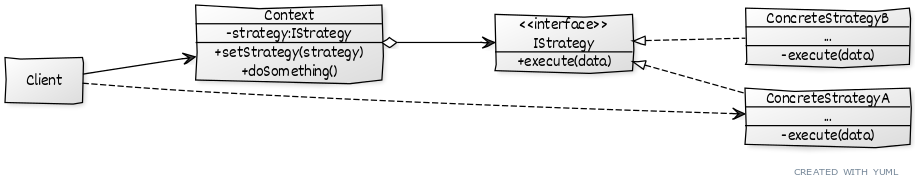
\includegraphics[width=0.9\linewidth]{images/StrategyUml}
	\caption{Diagram UML wzorca Strategia.}
	\label{lab2/fig/AbstractFactoryUml}
\end{figure}
%[Client]->[Context]
%[Client]-.->[ConcreteStrategyA]
%[Context]<>->[IStrategy]
%[IStrategy]^-.-[ConcreteStrategyA]
%[IStrategy]^-.-[ConcreteStrategyB]
%
%[Client]
%[Context|-strategy:IStrategy|+setStrategy(strategy);+doSomething()]
%[≪interface≫;IStrategy|+execute(data);]
%[ConcreteStrategyA|...|-execute(data)]
%[ConcreteStrategyB|...|-execute(data)]

\subsection{Iterator(ang. iterator)}
